\documentclass[12pt]{article}
\usepackage[utf8]{inputenc}
\usepackage[T1]{fontenc}
\usepackage[left=2cm,right=2cm,top=2cm,bottom=2cm]{geometry}
\usepackage[french]{babel}
\usepackage{graphicx}
\usepackage{url}
\usepackage{hyperref}

\hypersetup{
    colorlinks,
    citecolor=black,
    filecolor=black,
    linkcolor=black,
    urlcolor=black
}
\bibliographystyle{alpha}

\begin{document}

	\begin{titlepage}
		
\includegraphics[scale=0.2]{logo_bordeaux.png}\\
		\centering
		\linebreak
		{\LARGE \bfseries Université de Bordeaux}\\ [2cm]
		\textsc{\Large Master 1 Informatique}\\ [0,3cm]
		\textsc{\Large 2016/2017}\\ [1,4cm]

		\textsc{\Large Projet de programmation}\\ [1.4cm]

		\rule{16cm}{1mm}\\ [0,7cm]
		{\huge \bfseries Mémoire}\\ [0,5cm]
		{\huge \bfseries Visualisation d'un système de vélos en libre service} \\[0,7cm]
		\rule{16cm}{1mm}\\ [1cm]

		{\Large Chargé de TD Boris MANSENCAL }\\ [0,3cm]
		{\Large Client Romain GIOT }\\ [1cm]

		{\Large Damien Bielawski }\\ [0,3cm]
		{\Large Sébastien Bielawski }\\[0,3cm]
		{\Large Alaric Braillon }\\ [0,3cm]
		{\Large Alassane Diop }\\ [2cm]
		\Large\today

	\end{titlepage}

 
\tableofcontents \newpage

\section*{Remerciements} 
	Nous tenons à remercier Mr. Mansencal notre chargé de TD, ainsi que notre client Mr. Giot
	pour le temps qu'ils nous ont consacré. Ils nous ont été d'une aide précieuse, notamment
	sur des conseils portés au niveau de la direction à suivre sur les choix des structures de
	données	par exemple.
	
	
	\newpage
\part{Introduction}

	\section{Présentation du projet}
	Le projet consiste à développer une application qui doit permettre de visualiser
	un système de vélo en libre service. Le système de vélos en libre service se répand
	de plus en plus dans les grandes villes. Ainsi, pour mieux comprendre les habitudes
	des utilisateurs mais aussi pour faire des analyses statistiques, nous avons
	développé une logiciel qui permet de visualiser des trajets réalisés par des personnes
	ayant utilisées des vélos en libre service. Grâce à celui-ci on peut aussi y voir les
	stations répertoriées. L'élément important est le système de filtre que le logiciel offre,
	grâce à celui-ci, on peut afficher par des courbes, les trajets et stations que l’on
	souhaite. On peut également filtrer sur les heures ou les types de trajets (entrant ou
	sortant) par exemple. \\

	L’application doit charger en ensemble de données via un fichier. Notre logiciel doit se
	baser sur un travail réalisé par une équipe de chercheur,
	nommer les chercheurs qui ont rédigé un article le citer et mettre un lien. Ils ont
	aussi mis à disposition une courte vidéo montrant leur application web. Il est en revanche
	pas possible de la testé. Le fait que cette application soit faite pour le web, on peut
	supposer qu’elle soit limitée au niveau des performances,  qu’elle soit relativement
	lente lorsqu’il s’agit de traiter des millions de trajets. C’est la raison pour laquelle 
	le projet consiste à développer une application de bureau.
	
	\section{Étude de l’existant}
	L’application proposée par les chercheurs est divisée en trois fenêtres principales.
	La première permet de naviguer sur une carte d’une ville. Elle permet de voir les
	stations et les trajets sélectionnés par l’utilisateur à partir de la fenêtre centrale.
	Cette dernière, est une matrice qui contient les trajets pour chaque station, sur un
	interval de temps, 24 heures ici. Elle permet de sélectionner avec la souris un
	ensemble de glyphs (ensemble de trajet pour une station donnée et une heure donnée)
	ce qui permet de sélectionner une plage horaire ou tous les trajets d'une station par exemple.
	La troisième fenêtre, située à droite, met a disposition un ensemble de filtre modifiable
	par des tirettes ou des cases à cocher. \\

	\url{https://drive.google.com/file/d/0B3aeg8yMfRj0MWFmUHZ6ZlR4MzA/view}\\
	
	\url{https://drive.google.com/file/d/0B3aeg8yMfRj0R3VKQjdtX1htUUU/view}\\
	
	Quand on visionne la vidéo proposé par les chercheur, on peut s'apercevoir dans un premier
	temps, qu'elle l’application est lancée depuis Google Chrome. Son URL* (localhost :8080)
	nous indique qu’il s’agit d’une démonstration en local. Ne pouvant pas tester l’application,
	nous avons peu d’informations sur sa rapidité en fonction du nombre de données et la manière
	précise de son fonctionnement. Aussi, nous ne savons pas à quoi correspondent les jours de la
	semaine dans la partie filtre. En revanche, on peut supposer que les performances ne
	sont pas optimales avec ce type de technologie pour le web (on peut constater
	quelques lenteurs dans ses vidéos).\\
	Comme expliqué précédemment, notre projet avait pour
	but de reprendre les fonctionnalité de cette application.
	
	\section{Bibliographie}
		\begin{itemize}
			\item L'article \cite{Oli16} introduit clairement les problèmes rencontrés
			des systèmes de vélos en libre service. Notamment des problèmes d'équilibrage,
			de consommation de carburant pour les véhicules faisant la navette pour
			rééquilibrer les stations de vélos. On peut y puiser une grande source
			d'informations pour réaliser notre interface graphique. Ce sera le document sur
			lequel nous nous reposerons le plus.

			\item L'article \cite{Ali14} explique comment détecter les stations les plus
			connectées. Il donne un aperçu sur  l'utilisation des filtres (date, lieu, heure...).

			\item \cite{BC16} est un article sur les systèmes de partage de vélos. Il parle
			de l'application FunFEM qui permet de visualiser des données afin de juger de
			l'efficacité de ces systèmes.

			\item \cite{BSM17} est une application en ligne, qui permet de visualiser en
			temps réel des statistiques sur des bornes disponible dans une ville
			sélectionnée.  Elle indique également le nombre de vélos disponibles dans le
			monde en temps réel.

			\item L'article \cite{BW} de Ben Wellington, nous donne un bel aperçu sur la
			manière dont l'analyse statistique des données sur les utilisateurs du système de
			vélos en libre service peut être utilisée. Il montre comment les sociétés qui
			mettent à disposition les vélos dans la ville de New York pourraient augmenter
			leurs revenus grâce à une analyse des trajets des utilisateurs.

			\item \cite{JL} Recherches réalalisées sur la manière d'optimiser l'équilibrage
			des stations de vélos en libre service. Un des problèmes avec les stations de vélos
			est la gestion de l'équilibrage du nombre de  vélos dans chaque station. Il explique
			comment prédire à l'aide de données un épuisement de vélos dans certaines stations.
			Ainsi, à l'aide d'analyses d'une multitude de données sur la météo ou l'âge des
			utilisateurs par exemple, il est possible de d'optimiser la répartition des vélos et
			de faire des prédictions.

			\item Vidéo postée par Oliveira G \cite{state_station}, qui présente l'interface
			graphique de l'application web. Les différentes visualisations sont principalement
			portées sur l'analyse statistique des stations dans une ville donnée.

			\item Vidéo postée par Oliveira G \cite{trips}, qui présente cette fois une
			interface portée sur l'analyse des trajets. On peut séléctionner différents types
			de filtres.
		\end{itemize}

\part{L'analyse des besoins}

	\section{Besoins non fonctionnels}
		\subsection{Interfaces}
		Le texte de l’interface graphique sera en anglais.

		\subsection{Affichage des trajets}
		Les trajets seront affichés sur la carte par des courbes depuis le points de départ du
		trajet jusqu’au point d’arrivée.

		\subsection{Performances}
		Afin d’assurer la fiabilité du logiciel, des tests unitaires seront réalisés avec
		Banditcpp.\\
		"Bandit est un framework pour C++ 11 développé pour faire des tests unitaires. Bandit est
		l’en-tête seulement, donc il n’est pas nécessaire de compilation supplémentaire avant de
		pouvoir commencer à l’utiliser. Bandit a été testé avec les compilateurs suivants :
		GCC 4.5, GCC 4.6, GCC 4.7, GCC 4.8, Clang 3.2, VS2012.
		Bandit est libéré sous licence MIT. \\
		Bandit est livré avec un projet cmake pour générer des
		auto-tests bandit."
		(\url{http ://www.banditcpp.org/})\\
	
		L’application devra en priorité, tourner aussi sur une carte NVIDIA, elle doit aussi,
		sur demande du client, s’exécuter sur une carte graphique Quadro K2000M.\\
		
		On peut distinguer plusieurs attentes de rapidité en fonction des fonctionnalités :
		Lors de la lecture du fichier, le délai d’attente peut être long car il y a
		beaucoup de données à charger, on peut estimer ce délai à quelques secondes voire
		quelques minutes. \\
		
		Lors de l’application des divers filtres, le délai dois être assez court car 
		de ces filtres est assez récurrente.
		Lors du déplacement sur la carte et donc du rafraîchissement des données de celle-ci,
		le programme doit tourner en temps réel et on ne doit pas sentir de latence lors du
		déplacement sur la carte. Le délai doit donc être très court (dans l’ordre des millisecondes).\\
		Le code devra être très bien documenté, pour cela on utilisera Doxygen.
		"Doxygen est l’outil standard de facto pour générer de la documentation à partir de
		sources C++ annotées, mais il prend également en charge d’autres langages de
		programmation populaires.\\
		Il peut générer un navigateur de documentation en ligne (en HTML) et/ou un manuel de
		référence hors ligne à partir d’un ensemble de fichiers sources documentés. Il est
		également possible de générer des résultats en format RTF (MS-Word), PostScript,
		PDF hypertexte, HTML compressé et pages de manuel Unix. La documentation est 
		extraite directement des sources, ce qui rend beaucoup plus facile de conserver
		la documentation conforme au code source. \\
		Doxygen est développé sous Mac OS X et Linux, mais est configuré pour être très
		portable."\\
		
		\url{http ://www.stack.nl/ dimitri/doxygen/index.html} \\
		
		La dernière version de Qt sera utilisée, à l’heure actuelle, c’est la version
		5.8 stable.\\
		Pour le rendu graphique, la version d’OpenGL doit être supérieure à la version 3.2.
		Ainsi, aucune fonction obsolète ne sera utilisée.\\
		Le code C++ sera compilable avec le compilateur g++ 4.9.
		

	\section{Besoins fonctionnels}
		\subsection{Visualisation de la carte de la ville}
		Une fenêtre sur la partie gauche sera dédiée pour visualiser les trajets de
		manière géographique avec une carte.\\
		La carte d’une ville pourra être chargée avec OpenStreetMap\\
		La carte affiche uniquement les stations de la ville lorsqu’il y a des stations
		sélectionnées dans la matrice de chronologie, elle n’affiche que celles-ci (ainsi
		que les trajets qui y sont associés).\\
		Les trajets sont dessinés par des courbes avec un dégradé de deux couleurs.\\
		Les départs sont dessinés du cyan (station d’origine) vers le bleu (station de
		destination) dans le sens horaire.\\
		Les arrivées sont dessinées du rouge (station d’origine) vers le jaune
		(station de destination) dans le sens anti-horaire.\\
		Lorsque l’utilisateur passe sa souris sur une station de la carte, la ligne associée
		à la station est surlignée en noir dans la matrice de chronologie des trajets.\\
		Lorsque l’utilisateur passe sa souris sur une station de la matrice de chronologie
		des trajets, la station est surlignée en noir sur la carte.\\
		L’utilisateur pourra faire un zoom avant ou un zoom arrière grâce à la molette de la
		souris.\\
		Il pourra aussi se déplacer dans la carte, à gauche, à droite, en haut et en bas. Il
		réalisera cette action soit en appuyant sur des boutons, soit grâce à un système
		de glisser/déposer, afin de permettre une translation et se déplacer dans la carte.\\
		
		\subsection{Matrice de la chronologie des trajets}
		Axe horizontal : temps en heure (une colonne pour chaque heure)\\
		Axe vertical : stations (une ligne pour chaque station) les stations sont représentées dans
		des cellules par des petites étoiles (les lignes étant les trajets, représentés
		avec leurs directions et leur longueur)\\
		Arrivées en rouge\\
		Départs en bleu\\
		Trajets cycliques par des cercles transparents dont le rayon est proportionnel à
		la distance du trajet\\
		Possibilité de sélectionner les stations avec la souris, selon une intervalle horaire
		Les stations sélectionnées dans cette fenêtre sont visibles sur la carte, avec
		les trajets qui y sont associés\\
		Possibilité de dérouler, sur 24 heures, l’activité des emprunts des vélos
		en lançant l’animation (en appuyant sur le bouton play)\\
		
		\subsection{Interface de sélection des filtres}
		Possibilité de pouvoir filtrer dans le temps\\
		Un mois et son année : menu déroulant avec choix chargés à partir de fichiers
		données\\
		Un jour précis : entrée du jour du mois (un entier compris 1 et 31) dans un champ
		de texte\\
		Jour de la semaine/jours ouvrés/weekend\\
		Possibilité de filtrer selon les propriétés des trajets\\
		Arrivées : si cochée, affiche (en rouge) les trajets arrivants, sur la carte ainsi
		que dans la chronologie des trajets\\
		départs : si cochée, affiche (bleu) les trajets partant, sur la carte ainsi que
		dans la chronologie des trajets\\
		trajets cycliques : si cochée, affichés (par un cercle gris transparent dont le
		rayon est proportionnel à la longueur du trajet) les trajets cycliques, dans la
		chronologie des trajets\\
		durées des trajets : si cochée, prend en compte la durée des trajets\\
		longueurs des trajets : si cochée, prend en compte la longueur des trajets
		(les longueurs des traits des trajets dans chaque cellule de la chronologie des
		trajets sont relatives au trajet le plus long), sinon, tous les traits sont de même longueur\\
		Filtrer selon des valeurs entières comprises dans un intervalle borné par une
		valeur minimale et une valeur maximale\\
		longueur (en mètres)\\
		durée (en secondes)\\
		direction (en degrés)\\
		flux d’origine-destination\\		
	
	\section{Scénarios}
	
	\section{Prototype}
	Pour la remise de la 1er release, nous avons voulu de rendre un programme qui permettait
	d'afficher des stations et des trajets ainsi qu'un aperçu de ce que cela pourrait rendre
	dans la timelinematrix. Ayant un temps très court pour réaliser cela, nous avons testé
	d'afficher ces éléments avec les objets que Qt5 nous met à disposition.\\
	

	\begin{figure}[!h]
	\begin{center}
	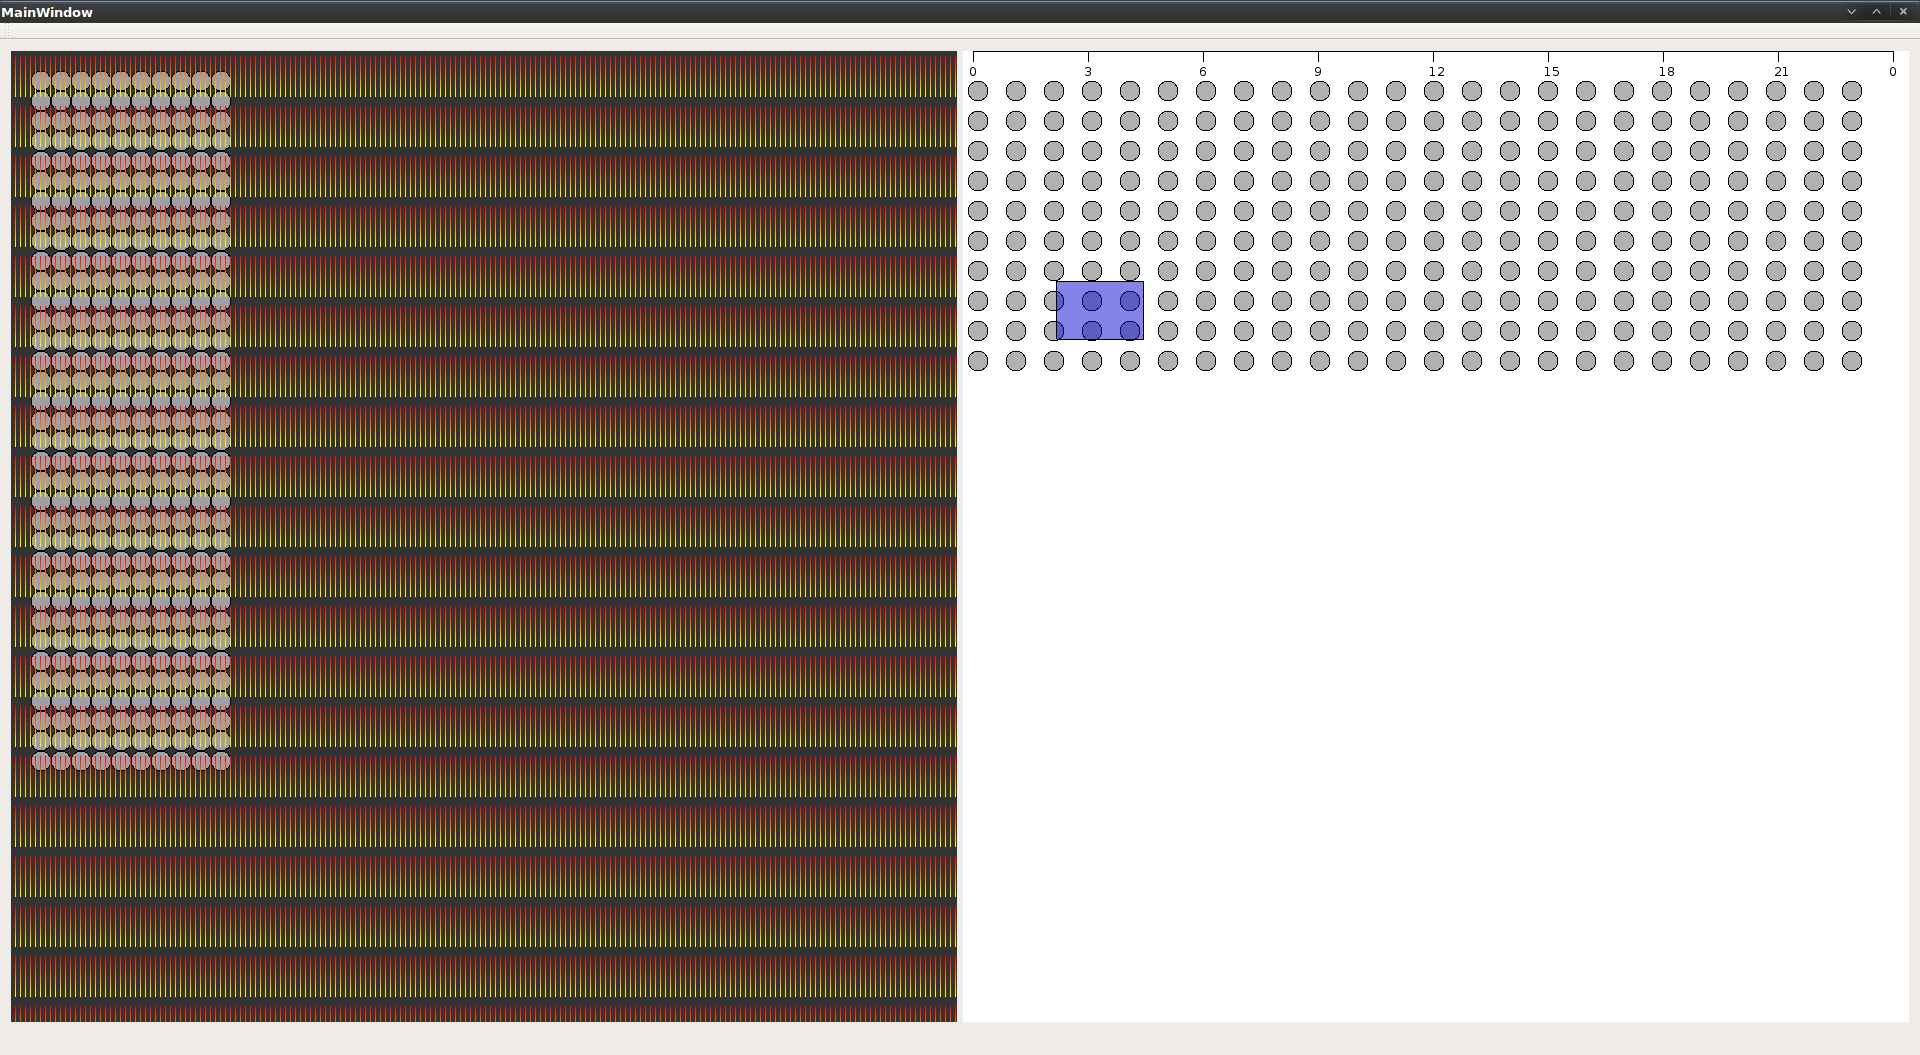
\includegraphics[scale=0.2]{prototype1_screen_shot.png}
	\caption{Prototype de la première release}
	\end{center}
	\end{figure}		
	
	Ce prototype nous a permis de nous rendre compte que l’utilisation des objets Qt pour
	dessiner les trajets et stations ne satisfera pas les attentes des besoins non
	fonctionnels. C’est la raison pour laquel, malgré les difficultés rencontré
	nous avons utilisé OpenGL pour le rendu.\\
	
	Des tests de performances ont été réalisé sur ce prototype et se trouve plus bas.\\

\part{L'architecture}

	\section{Architecture générale}
		\subsection{Architecture 3-tiers}
		L’architecture se compose de trois couches :
		\begin{itemize}
			\item couche présentation
			\item couche métier 
			\item couche accès aux données
		\end{itemize}
			
		L'utilisateur manipule le logiciel avec les contrôles (boutons, sliders à deux
		poignées et menu déroulant) de l’interface graphique. Ce seront, concrètement,
		des opérations de filtrages et de sélection des trajets, ainsi que de filtrage
		et de tri des stations. C’est dans cette couche que ces opérations sont appelées. \\
		
		Le contrôleur de l’interface manipule les données du modèle. C’est dans cette
		couche que les opérations demandées par l’utilisateur au 1) sont exécutées.\\
		
		(dans notre cas, le modèle n’écris pas sur les données, l’accès des données se
		fait en lecture seule)\\
		
		Le modèle accède aux données. Ici, le modèle ne fait que parser des fichiers,
		sans les modifier. Le fichiers sont refermés une fois l’opération de parsing
		terminée. Le modèle charge les données en initialisant une liste pour les trajets,
		une autre pour les stations. Cela se fait à chaque fois que l’utilisateur
		souhaite charger un fichier\\
		
		Le modèle notifie l’interface graphique des résultats des opérations demandées
		depuis 1). Tous les composants graphiques concernés sont mis à jour, notamment la
		map affichant les trajets, ainsi que la matrice de chronologie des trajets.\\
		
		L’interface graphique affiche à l'utilisateur les résultats de ses requêtes.\\
		
		\begin{figure}[!h]
		\begin{center}
		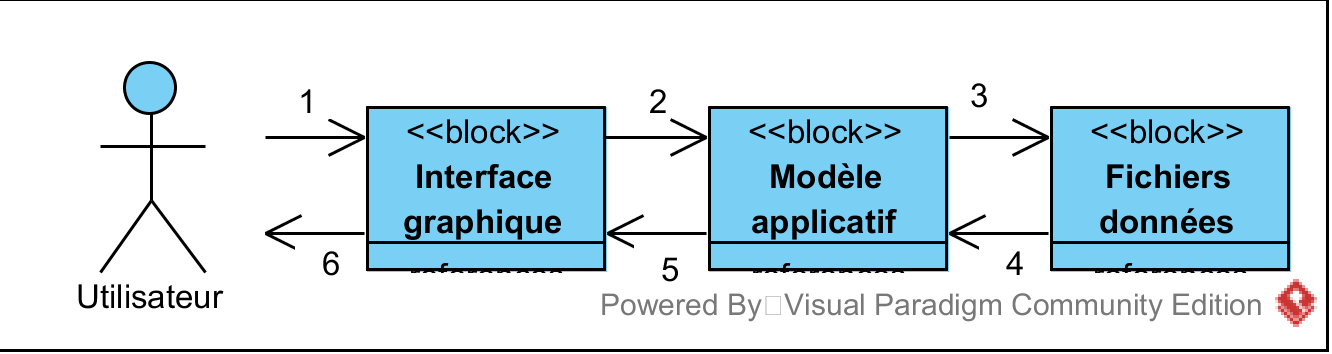
\includegraphics[scale=1]{dia_block_3tiers.png}
		\caption{Architecture 3-tiers}
		\end{center}
		\end{figure}

		\subsection{Architecture MVC}
		L’architecture du projet est basée sur le modèle MVC classique (Modèle/Vue/Contrôleur).\\
		
		Le Modèle :\\
		Anciennement appelé “Model”, il a été renommé en “Data”, car cette classe ne fait
		que contenir des données (les stations et les trajets), avec la possibilité de les
		charger et les décharger.\\
		
		La Vue :\\
		C’est l’ensemble des composants de l’interface graphique (les widgets). Ces
		widgets sont implémentés par Qt soit C++, soit en QML (pour Qt Modeling Language).
		Il sont contenus dans la classe “MainWindow”.\\
				
		Le Contrôleur :\\
		C’est la classe “MainWindow”, nom généré par le designer d’interface graphique
		de QtCreator. Elle est contenue dans l’espace de nom “Ui” (également généré par Qt).
		Elle joue le rôle de contrôleur en étant composée des composants graphiques ainsi
		que du modèle. Elle fait communiquer le Modèle et la Vue via le mécanisme
		des signaux implémenté par Qt. \\
		
		\begin{figure}[!h]
		\begin{center}
		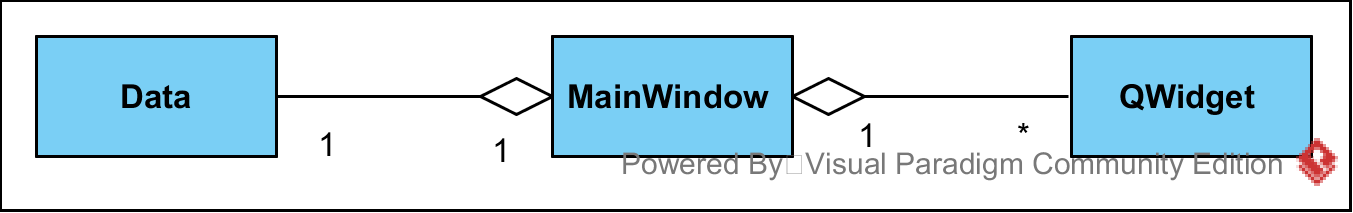
\includegraphics[scale=1]{dia_class_mvc.png}
		\caption{Relation des compositions des classes implémentant le MVC}
		\end{center}
		\end{figure}
		
		\subsection{Les packages}
		On distingue deux espaces de noms (voire trois si on considère que les classes de
		Qt sont contenues dans un espace de nom) (cf. Figure 1: Diagramme de package
		ci-dessous):\\
	
		\begin{itemize}
		\item l’espace de nom “Ui” (pour “User interface”), qui est généré par Qt. Il est utilisé
		pour y regrouper les composants graphiques qui sont auto-générés avec le designer
		d’interfaces graphiques. Le Contrôleur est également contenu dans “Ui”. La Vue et
		le Contrôleur sont donc gérés au niveau de “Ui”. “Ui” dépend de “bss” et des
		classes de Qt.\\
		
		\item l’espace de nom “bss” (pour “Bike Sharing System”), qui contient les
		classes du Modèle. “bss” utilise des objets et des fonctions de Qt en plus de
		ceux proposés par C++ 14.
		\end{itemize}

		\begin{figure}[!h]
		\begin{center}
		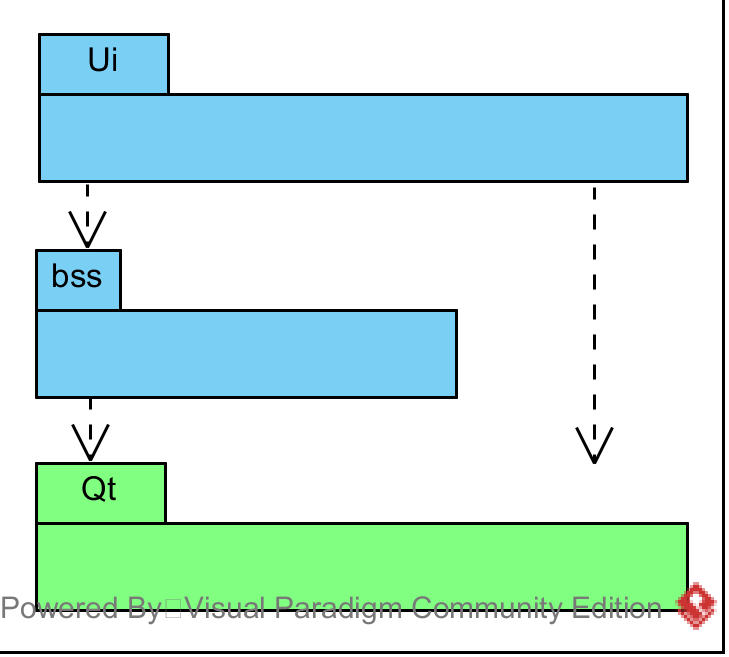
\includegraphics[scale=1]{dia_package.png}
		\caption{Diagramme de package}
		\end{center}
		\end{figure}
		
		\subsection{Représentation des données (trajets et stations)}
		Les données à manipuler sont représentés par des structures aux attributs publics,
		initialisés lors du parsing des fichiers. Ces entités sont passives, elles ne possèdent
		pas de méthodes qui produisent ou modifient d’autres objets. Ce sont donc des
		“classes-enregistrement” qui ne font que structurer la représentation des données.\\
		
		
		Trip :\\
		Cette structure contient les données nécessaires au filtrage et sélection des trajets :\\		
		\begin{itemize}
			\item[•]ses temps de départ et d’arrivée (comprend la date ainsi que l’heure)
			\item[•]sa durée (en secondes, codée par un entier sur 64 bits, initialisée à 0 par défaut)
			\item[•]sa distance (en mètres, codée par un entier sur 64 bits, initialisée à
			0 par défaut)
			\item[•]sa direction (ou azimut, en degrés, codée sur un réel, initialisée à 0 par défaut)
			\item[•]un flag pour indiquer s’il est cyclique ou non (faux par défaut)\\
		\end{itemize}
		
		
		Station :\\
		Cette structure contient les données nécessaires au filtrage et tri des stations :\\
		\begin{itemize}
			\item[•]son nom (sous forme de chaîne de caractères)
			\item[•]ses coordonnées géographiques (latitude et longitude) (en degrés,
			des réels initialisés à 0)
			\item[•]la distance moyenne (en mètres) d’un trajet (un entier, qui vaut 0 par défaut)
			l\item[•]a durée moyenne (en secondes) d’un trajet (un entier, qui vaut 0 par défaut)
		\end{itemize}
		
		\subsection{Association entre les stations et les trajets}
		Un trajet est obligatoirement associé à deux stations : celle d’arrivée et celle
		de départ. L’association ne se fait pas de manière classique avec des pointeurs mais avec des
		identifiants. Ces identifiants sont codés par des entiers. L’idée au départ était de les
		coder sur entiers.

		\begin{figure}[!h]
		\begin{center}
		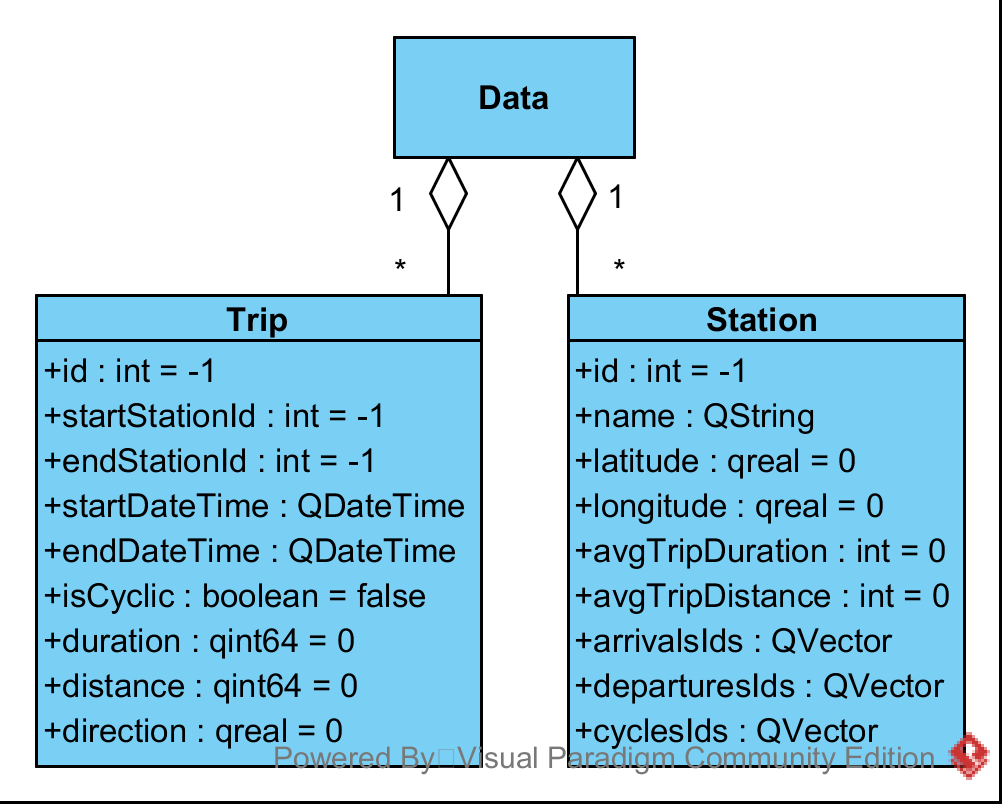
\includegraphics[scale=1]{dia_class_data.png}
		\caption{Représentation des structures de données}
		\end{center}
		\end{figure}
		
		\subsection{La classe “DataFileReader”}
		C’est une classe qui est utilisée localement par la classe “Data” pour parser et
		charger les données. Elle hérite de la classe “AbstractDataFileReader”, qui définit
		les prototypes des méthodes de parsing des données. “DataFileReader” utilise en
		interne des parseurs spécialisés (qui héritent également de la classe abstraite) selon
		le type du fichier : elle utilisera :
		\begin{itemize}
			\item[•]un “CsvDataFileReader” pour parser un fichier CSV
			\item[•]un “XmlDataFileReader” pour parser un fichier XML
			\item[•]un “JsonDataFileReader” pour parser un fichier Json
		\end{itemize}

		Le résultat retourné par une opération de parsing retourne une structure
		“DataFileReadInfo” qui contient une chaîne de caractère, ainsi qu’un flag
		(mis à “vrai” si l’opération est un succès, “faux” sinon, auquel cas, la chaîne
		de caractère contient le message d’erreur).\\
		Ce résultat est transmis à la classe “Data”.
		
		\subsection{La classe “Data”}
		C’est la classe principale. Elle permet de charger les données (via un”DataFileReader”)
		à partir d’un nom de fichier spécifié, et de gérer l’allocation mémoire de ces données.
		Les données chargées sont contenues de manière contiguë dans des objets de type “QVector”
		(c’est le conteneur de premier choix, selon la documentation de Qt).
		Une fois les données chargées, elle garantit leur accès en lecture seule au Contrôleur,
		pour permettre les opération de filtrages sur les trajets. Un signal “dataLoaded” est
		émis lorsque les données ont été chargées avec succès. Un signal “failedToLoad” est
		émis lorsque le chargement est un échec. Elle retourne une structure “DataLoadResult”
		qui contient une chaîne de caractère, les données (si chargées) et un flag (mis à “vrai”
		si le chargement via le parseur est un succès, “faux” sinon, auquel la chaîne de
		caractère contient le message d’erreur).

	\section{Modules}

\part{Les tests}

	\section{Les tests de performances}
		\subsection{Conditions de tests}
		Les tests ont été réalisés sur un système d’exploitation Linux Debian 8.7 avec
		un noyau de version 3.16.0-4-amd64. \\ \\
		Spécifications de la machine: \\
		\begin{center}
			\begin{tabular}{| l | c |}
			\hline
			\textbf{Composants} & \textbf{Model} \\ \hline
			Processeur & Intel I5 2500k \\ \hline
			Carte Graphique & NVIDIA GTX 970 4Go \\ \hline
			Mémoire vive & 12 Go \\ \hline
			Disque dur & à 7200 trs/min \\ \hline
		    \end{tabular}
	    \end{center}
	    
	    Outils de développement: \\
	    \begin{center}
			\begin{tabular}{| l | c |}
			\hline
			\textbf{Outils} & \textbf{Version} \\ \hline
			gcc & 4.9.2 \\ \hline
			Qt & 5.8 \\ \hline
			Flags de compilation & C++14\\ \hline
		    \end{tabular}
	    \end{center}
	    
	    Le fichier utilisé pour tester les temps de chargement est disponible à ce lien:\\
		\url{https://s3.amazonaws.com/tripdata/201310-citibike-tripdata.zip}\\
		
		Le fichier contient 843 416 trajets et 329 stations.
	    
		\subsection{Chargement des fichiers en mémoire}
		
		\begin{center}
			\begin{tabular}{| l | c |}
			\hline
			\textbf{Méthode} & \textbf{temps (en millisecondes)} \\ \hline
			Séquentiel & 21 214 \\ \hline
			Parallèle & à tester \\ \hline
		    \end{tabular}
	    \end{center}
		
		\subsection{Affichage des trajets et des stations}
		\begin{center}
			\begin{tabular}{| l | c |}
			\hline
			\textbf{Méthode} & \textbf{temps (en millisecondes)} \\ \hline
			QPainter & 1396 \\ \hline
			OpenGL & 1 \\ \hline
		    \end{tabular}
	    \end{center}
	    	    
		\subsection{Affichage des glyphs}
		\begin{center}
			\begin{tabular}{| l | c |}
			\hline
			\textbf{Méthode} & \textbf{temps (en millisecondes)} \\ \hline
			QPainter & Non testé\\ \hline
			OpenGL & 1 \\ \hline
		    \end{tabular}
	    \end{center}
		
	\section{Les tests boite blanche}
	
	\section{Les tests boite noire}
	
	\subsection{Analyse de fonction}
	L’outil Valgrind nous a permis de réaliser plusieurs tests, notamment des tests sur les
	fonctions avec Callgrind, lors de l'exécution de notre programme. Ci dessus, une
	impression écran du résultat de notre analyse.
	
	\begin{figure}[!h]
	\begin{center}
	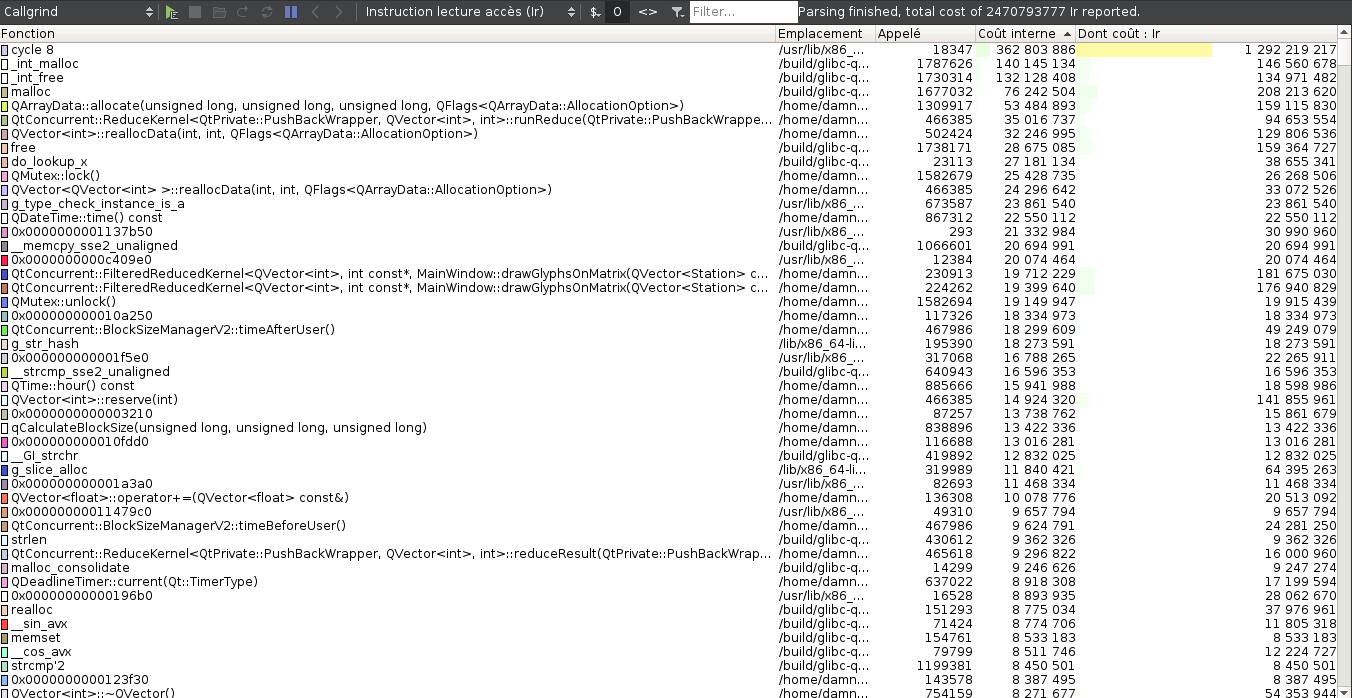
\includegraphics[scale=.35]{callgrind_analyse.png}
	\caption{Analyse de fonctions avec Callgrind}
	\end{center}
	\end{figure}
	
	Pour réaliser cette analyse nous avons compilé en mode “Release” afin d’avoir un code optimisé.
	Sur cette analyse on peut voir que les fonctions les plus lourdes sont les fonctions
	parallélisées notamment drawGlyphsOnMatrix. L’allocation des QVector<QVector<int>>
	prend aussi beaucoup de temps . On notera aussi QDateTime::time.
		
	\subsection{Fuite de mémoire}
	Pour les fuites de mémoire nous avons aussi utilisé Valgring avec l’option
	valgrind --leak-check=full ./VisualBSS
	Comme on pouvait s’y attendre, l’API Qt génère de la fuite de mémoire
	lorsqu’on lance l’application.
	Nous avons en revanche pas trouvé de fuite mémoire venant de notre code.
	
	\begin{figure}[!h]
	\begin{center}
	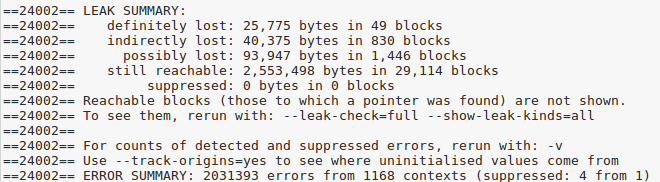
\includegraphics[scale=.5]{memory_leak.png}
	\caption{Test des fuites de mémoire avec Vallgrind}
	\end{center}
	\end{figure}

\part{Bilan}

	\section{Bugs présents}
		
	
	\section{Les difficultés rencontrées}
	Pour réaliser ce projet nous devions nous appuyer sur le document rédigé par le groupe de
	chercheur, ainsi que la vidéo. Pour réaliser notre cahier des besoins, il nous a été
	difficile de définir certains besoins car il nous manquait des informations ou précisions.
	De même pour l’application montrée dans la vidéo, nous ne pouvions pas la tester car nous
	n'avions pas accès.\\

	Concernant la réalisation de l’affiche avec OpenGL, nous somme resté bloqué plusieurs jours
	sur un bug. Cela nous a fait perdre beaucoup de temps.\\

	Durant le phase de développement, nous avons perdu du temps également à cause de la
	stratégie à adopter pour stocker les trajets et les stations. Nous avons essayé de faire
	simple et performant. Cela nous a valu de changer le code et de faire des tests pour savoir
	si les performances serait présente.\\
	
	\section{Critiques}
	Nous ne devrions pas stocker des identifiants dans les QVector, cela ralentit notre
	l’application à cause des conversions entre les id et les stations/trajets. Nous pensons que
	nous aurions dû utiliser des shared pointer.\\
	Les ralentissements que cela occasionne nous a contraint à réduire l’interactivité de
	notre application en mettant à jour les trajets sélectionnés dans la timelinematrix qu’une
	fois que l’utilisateur ait relâché le bouton gauche de la souris. 
	
	\section{Conclusion}

	\newpage
	\section{Lexique}
	\begin{itemize}
		\item[]\textbf{BSS} : bike sharing system, système de vélos en libre service\\
		\item[]\textbf{CSV} : CSV : Comma Separated Value, c'est un format de fichier\\
		\item[]\textbf{XML} :\\
		\item[]\textbf{JSON} : Java Script Object Notation, format de fichier\\
		\item[]\textbf{Qt} : Est un framework très populaire pour le développement
		d'interfaces graphiques\\
		\item[]\textbf{Test en boite blanche} : \\
		\item[]\textbf{Test en boite noire} :  \\
		\item[]\textbf{Doxygene} : Outil permettant de générer de la documentation,
		au format html ou en Latex par exemple.\\
		\item[]\textbf{Glyph} : Un glyph est un élément de la timelinematrix, elle
		représente un ensemble de trajet d'une station donnée est d'une heure donnée.\\
		\item[]\textbf{shared pointer} :\\
	\end{itemize}

	\newpage
	\listoffigures
	
	\newpage
	\section{Annexes}

	\bibliography{bibliographie}
 
\end{document}